\documentclass{article}
\usepackage{../fasy-hw}
\usepackage{ wasysym }

%% UPDATE these variables:
\renewcommand{\hwnum}{5}
\title{Advanced Algorithms, Homework \hwnum}
\author{Nathan Stouffer}
\collab{n/a}
\date{due: 15 October 2020}

\begin{document}

\maketitle

\nextprob
\collab{n/a}

You should make at least ten contributions to the Piazza board
discussing the solutions to Problems in Chapter 5 or 6 of the textbook.  Your
contribution does not have to be a complete solution.  It can be any element of
a full solution to a problem requiring an algorithm as an answer.  (For this
question, the outcomes are: insufficient posts (-1), low pass (+1), pass (+3),
and high pass (+5).

Caveat: The number of contributions that can count from a single day are the
number of days before the assignment is due +1.  (So, Thursday the 15th, you can
have one post count, the day before two, etc.)

\paragraph{Answer}

% ============================================

My contributions are:
\begin{enumerate}
    \item (Chapter 6 Question 5 at 12:45 pm on 10/09/2020). \\
        An edge $e$ in a connected undirected graph $G$ is called a bridge (or a cut edge) if the subgraph $G - e $ (obtained by removing $e$ from $G$) is disconnected.
        \begin{enumerate}[label=(\alph*)]
            \item Given $G$ and edge $e$ describe a linear-time algorithm that determines whether $e$ is a bridge or not. What is the running time to find all bridges by trying your algorithm for each edge?
            \item Let $T$ be an arbitrary spanning tree of $G$. Prove that every bridge of $G$ is also an edge in $T$. This claim implies that $G$ has at most $V-1$ bridges. How does this information improve your algorithm from part (a) to find all bridges?
            \item Now suppose we root $T$ at an arbitrary vertex $r$. For any vertex $v$, let $T_v$ denote the subtree of $T$ rooted at $v$; for example, $T_r = T$. Let $uv$ be an arbitrary edge of $T$, where $u$ is the parent of $v$. Prove that $uv$ is a bridge of $G$ if and only if $uv$ is the only edge in $G$ with exactly one endpoint in $T_v$ .
            \item Describe a linear-time algorithm to identify every bridge in $G$. [Hint: Let $T$ be a depth-first spanning tree of $G$.]
        \end{enumerate}
    \item (Chapter 6 Question 5 at 11:00 am on 10/10/2020). \\
        For part a, we are given a graph $G$ and and edge $e$. From there, we must determine if $e$ is a bridge for $G$ in linear time. To do this, we can use the following pseudocode.

        \begin{algorithm}
            IsBridge(G, e) \\
            $\cdot$ \hspace{1em} src = source(e) \\
            $\cdot$ \hspace{1em} trg = target(e) \\
            $\cdot$ \hspace{1em} H = G - e \\
            $\cdot$ \hspace{1em} dfs(H, src) \\
            $\cdot$ \hspace{1em} if (trg is not marked in H): \\
            $\cdot$ \hspace{2em} return True \\
            $\cdot$ \hspace{1em} return False \\
        \end{algorithm}

        Every line in the above algorithm (except for $dfs(H, src)$) runs in constant time. We know that first search runs in $O(V + E)$ time so the $IsBridge()$ runs in linear time. The algorithm is correct because depth first search marks all vertices that are reachable from a source vertex. We are running depth first search on the graph H, which does not contain our query edge $e$. So if we do not mark $trg$ in depth first search, then $H$ (which is $G$ without $e$) is disconnected.

        As far as the running time to find all bridges, we must call $IsBridge$ on each edge in the graph $G$. So the runtime is $EO(V + E) = O(EV + E^2)$.
    \item (Chapter 6 Question 5 at 10:30 pm on 10/12/2020). \\
        I was thinking that a proof by contradiction would fit nicely here.

        Claim: Let $G$ be a connected graph, and let $T$ be an arbitrary spanning tree of $G$.
        Every bridge of $G$ is also an edge in $T$.

        Proof: Let $G = (V, E)$ be a connected graph with spanning tree $T = (V_T, E_T)$.
        Let $e$ be a bridge in $G$.
        Now suppose that $e$ is not in $T$ ($T \subset G - e$).
        Since $T$ is a spanning tree, $T$ contains a path from every $u \in V$ to every $v \in V$.
        But this is a contradiction since $T \subset G - e$ and $G- e$ is disconnected (so some vertices exist with no paths between them).
        Since we reached a contradiction by assuming that $e$ is not in $T$, that must have been an incorrect assumption.
        So it must have been true that $e$ is in $T$.
    \item (Chapter 6 Question 15 at 11:30 pm on 10/12/2020). \\
        A polygonal path is a sequence of line segments joined end-to-end; the endpoints of these line segments are called the vertices of the path.
        The length of a polygonal path is the sum of the lengths of its segments.
        A polygonal path with vertices $(x_1, y_1), (x_2, y_2), ... ,(x_k, y_k)$ is monotonically increasing if $x_i < x_{i+1}$ and $y_i < y_{i+1}$ for every index $i$ --- informally, each vertex of the path is above and to the right of its predecessor.

        Suppose you are given a set $S$ of $n$ points in the plane, represented as two arrays $X[1 .. n]$ and $Y [1 .. n]$.
        Describe and analyze an algorithm to compute the length of the longest monotonically increasing path with vertices in $S$.
        Assume you have a subroutine $L(x, y, x_0, y_0)$ that returns the length of the segment from $(x, y)$ to $(x_0, y_0)$.
    \item (Chapter 6 Question 15 at 10:40 am on 10/13/2020). \\
        The problem already gives some description of input.
        We are given $n$ points in the plane in the form of two arrays: $X[1..n]$ and $Y[1..n]$.
        Suppose we preprocess the input as follows before calling our algorithm.
        The function $SortByX$ sorts the array of $X$ coordinates but preserves the parrallel property of the arrays $X$ and $Y$.

        \begin{algorithm}
            \textsc{LongestPolygonalPath}(X[1..n], Y[1..n]) \\
            $\cdot $ \hspace{1em} X, Y = SortByX(X, Y) \\
            $\cdot $ \hspace{1em} L[1..n] = [ -inf, -inf, ..., -inf ] \\
            $\cdot $ \hspace{1em} return LPP(X, Y, 0)
        \end{algorithm}

        We can implicitly represent the underlying graph with the following rules. Given an $k$, we can draw an edge from the point $(X[k], Y[k])$ to every point $(X[i], Y[i])$ where $i > k$ and $Y[i] \geq Y[k]$. In words, since $X$ is sorted we can't select any point with index less than $k$. Additionally, we need to check that the point we select does not have a lower $Y$ coordinate than our previous point (this would violate monotonically increasing).

        Now that we have established the underlying graph, we can run the following algorithm. In this algorithm, we compute every possible monotonically increasing sequence and return the path with the longest length. Note that $k$ is the index of the most recently added vertex to the path.
        \newpage
        \begin{algorithm}
            \textsc{LLP}(X, Y, k) \\
            $\cdot $ \hspace{1em} x = X[k] \\
            $\cdot $ \hspace{1em} y = Y[k] \\
            $\cdot $ \hspace{1em} max  = 0 \\
            $\cdot $ \hspace{1em} test = 0 \\
            $\cdot $ \hspace{1em} for i in k+1..n // check all possible outgoing edges \\
            $\cdot $ \hspace{1em} if (Y[i] $\geq$ Y[k])	// make sure edge is monotonically increasing in Y \\
            $\cdot $ \hspace{2em} test = L(x, y, X[i], Y[i]) + \textsc{LLP}(X, Y, i) \\
            $\cdot $ \hspace{1em} if  (test $>$ max) \\
            $\cdot $ \hspace{2em} max = test \\
            $\cdot $ \hspace{1em} return max
        \end{algorithm}

        However, this run time is absolutely atrocious. I think this is what happens in the very worst case. The recurrence relation is $T(n) = n * T(O(n-1))$. The $n$ comes from the for loop and the $O(n-1)$ comes from the fact that, in the worst case, only the current point is now ineligible to be a part of the monotonically increasing path. So the run time is $O(n!)$ in the worst case.
    \item (Chapter 6 Question 15 at 12:40 pm on 10/13/2020). \\
        We can improve on this run time practically (although I am struggling to think of a theoretical improvement).
        Instead of the preprocessing used above, we should use the following preprocessor function that initializes a global array $L[1..n]$.
        This array stores the longest discovered path (subject to the constraints) to vertex $i$ in $L[i]$.

        \begin{algorithm}
        \textsc{LongestPolygonalPath}(X[1..n], Y[1..n]) \\
            $\cdot$ \hspace{1em} X, Y = SortByX(X, Y) \\
            $\cdot$ \hspace{1em} L[1..n] = [ -inf, -inf, ..., -inf ] \\
            $\cdot$ \hspace{1em} return max(L)
        \end{algorithm}

        Then our algorithm can perform an additional check to see if a longer path to the same vertex has already been discovered.

        \begin{algorithm}
            $\cdot$ \hspace{1em} LLP(X[1..n], Y[1..n], k) \\
            $\cdot$ \hspace{1em} x = X[k] \\
            $\cdot$ \hspace{1em} y = Y[k] \\
            $\cdot$ \hspace{1em} for i in k+1..n \\
            $\cdot$ \hspace{2em} if (Y[i] $\geq$ Y[k]) \\
            $\cdot$ \hspace{3em} if (L[k] + L(x, y, X[i], Y[i]) $>$ L[i]) \\
            $\cdot$ \hspace{4em} L[i] = L[k] + L(x, y, X[i], Y[i]) \\
            $\cdot$ \hspace{4em} LLP(X, Y, i)
        \end{algorithm}

        Practically, this new algorithm will not compute some paths that we know will not be the longest polygonal path because a longer one to the same vertex has already been discovered.
        However, this does not improve the theoretical bound of $O(n!)$.
    \item (Chapter 6 Question 15 at 11:40 pm on 10/13/2020). \\
        Hey Giorgio,

        I am confused as to why the path must be consecutive in the set $S$ (since the listing order in a set is not important).
        From the problem in the textbook, it seems like we are supposed to find the longest monotonically increasing sequence of points in $S$.
        It seems like the index $i$ refers to the index in the sequence, not the index of the arrays.
        The arrays $X$ and $Y$ are just a representation of the set $S$ but it could be put in any order.
        Let me know what you think.
    \item (Chapter 6 Question 15 at 2:15 pm on 10/14/2020). \\
        It is a fair point that the algorithm repeats some calculations. To solve this, we should fill out the array $L$ in an intelligent way. I don't think that my initial algorithm lends itself well to dynamic programming because $L$ doesn't explicitly depend on a recursive call that I can index (as far as I can tell). However, I do think that my algorithm naively uses depth first search instead of breath first search. Most of the time, we consider these algorithms to be the same (maybe we just care about connectivity). In this case, we want to find the maximum length path. Depth first search will compute the length of an entire path, regardless of whether it is the path we care about. On the other hand, breath first search (along with some special conditions about when to stop) would stop searching paths that do not have significant weight (I think).
    \item (Chapter 6 Question 5 at 2:22 pm on 10/14/2020). \\
        I can definitely be more specific. Here is my edited version of the proof.

        Claim: Let $G$ be a connected graph, and let $T$ be an arbitrary spanning tree of $G$.
        Every bridge of $G$ is also an edge in $T$.

        Proof: Let $G=(V,E)$ be a connected graph with spanning tree $T=(V_T,E_T)$.
        Let $e$ be a bridge in $G$ between vertices $w$ and $w'$ ($e = (w, w')$.
        Now suppose that $e$ is not in $T$ ($T \subset G - e$).
        Since $T$ is a spanning tree, $T$ contains a path from every $u \in V$ to every $v \in V$.
        But this is a contradiction since $T \subset G - e$ and $G - e$ is disconnected (some vertices exist with no paths between them, certainly $w$ and $w'$ are no longer connected since $e$ was their only connection).
        Since we reached a contradiction by assuming that $e$ is not in $T$, that must have been an incorrect assumption.
        So it must have been true that $e$ is in $T$.
    \item (Chapter 6 Question 6 at 6:12 pm on 10/15/2020). \\
        Problem description: The input to this algorithm is some directed graph $G = (V, E)$. The output of our algorithm will be a transitive closure of $G$. The transitive closure of $G$, is some graph $G^T = (V, E^T)$ where $E^T := \{ (u, w) \in V \mid$ there exists a path in $G$ from $u$ to $v \} $. 
\end{enumerate}

% ============================================

\nextprob
\collab{n/a}

Chapter 4, Question 1 (Greedy Schedule).  I encourage you to think through all 9
alternative schedules.  However, you only need to hand in two:
\begin{enumerate}
    \item Choose one alternate strategy that
        works, and prove that it works.
    \item Choose one alternate strategy that does not work, and give a
        counter-example.
\end{enumerate}

\paragraph{Answer}
% ============================================

\begin{enumerate}
    \item For a greedy scheduler strategy that works, I chose to prove that strategy (h) works.
    Strategy (h) says Let $x$ be the class with the earliest start time and let $y$ be the class with the second earliest start time:
    \begin{itemize}
        \item If $x$ and $y$ are disjoint, choose $x$ and recurse on everything but $x$
        \item If $x$ completely contains $y$, discard $x$ and recurse
        \item Otherwise, discard $y$ and recurse
    \end{itemize}
    To prove that this algorithm is correct, we must show that each case makes a correct choice and that the algorithm will terminate.
    Let's begin by showing that the first choice is a correct one.
    Suppose that $x$ and $y$ are disjoint.
    This implies that $x$ does not intersect with any other classes (since all other classes start after or equal to when $y$ starts).
    Since $x$ does not intersect with any other classes, it must be in the optimal schedule.
    So we should choose $x$ and continue on our way.

    We now show that if $x$ completely contains $y$, that we should discard $x$.
    If $y$ is contained completely in $x$, then any conflict with $y$ is surely a conflict with $x$.
    However, the converse is not true so we should discard $x$ because choosing $y$ is at least as good as choosing $x$.
    Therefore, we should discard $x$.

    Now we consider the final case: discard $y$.
    If we reach this case, then neither of the previous cases are true.
    So it must be true that $y$ starts before $x$ ends and that $y$ ends after $x$ ends.
    Then choosing $x$ is at least as good as choosing $y$ because any class that conflicts with $x$ will conflict with $y$ but the converse is not necessarily true.
    Therefore, we should discard $y$.

    The algorithm starts with the initial set of classs and then evaluates the pair $x$ and $y$.
    Note any configuration of the classes $x$ and $y$ must fall into one of the three given cases.
    After making a decision and acting (either choosing or discarding), the algorithm is called recursively on the remainder.
    Let's now prove that this algorithm terminates.
    Let our state space be the set of classes that are not chosen or discarded; we map this set to the natural numbers via cardinality.
    The function is strictly decreasing over each step in the recursion because each case either chooses or discards a class and every configuration of classes $x$ and $y$ falls into one of the cases.
    Therefore, at recursive step $i+1$, the cardinality of our state space is one less than that of recursive step $i$, which is strictly decreasing.
    Thus, the algorithm must terminate.

    Now we must prove the correctness of the entire algorithm.
    We do so by induction.
    The base case occurs at the beginning of the algorithm when no choices have been made.
    Then we make a choice that does not disagree with the optimal schedule (we know what this choice is via the proof of the three cases).
    Then we have made a single correct choice.
    For our inductive assumption, suppose that we have recursed $i \geq 1$ times and made a correct choice at each recursion.
    Now we must show that the $i+1$ recursion does not make an incorrect choice.
    But we have already shown that the three cases above outline a correct choice.
    So the $i+1$ choice must be made correctly and the inductive step is proved.

    So we have showed that the algorithm terminates and is correct.
    \item For an alternate strategy that does not work, I chose strategy (e).
    This strategy states that we should choose the course $x$ that conflicts with the fewest other courses, discard all classes that conflict with $x$, and recurse.
    This strategy fails with the following input:
    \begin{center}
        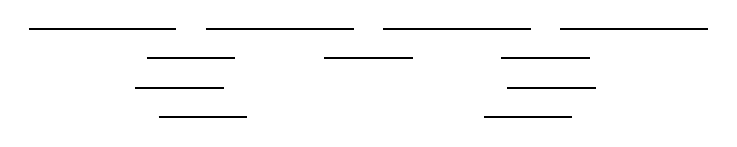
\begin{tikzpicture}[scale=1.5]
            % top 4
            \draw [thick] (-2.75, 0) -- (-1.5, 0);
            \draw [thick] (-1.25, 0) -- (0,    0);
            \draw [thick] (0.25,  0) -- (1.5,  0);
            \draw [thick] (1.75,  0) -- (3,    0);
            % middle
            \draw [thick] (-0.25, -0.25) -- (0.5, -0.25);
            % left
            \draw [thick] (-1.75, -0.25) -- (-1, -0.25);
            \draw [thick] (-1.85, -0.5) -- (-1.1, -0.5);
            \draw [thick] (-1.65, -0.75) -- (-0.9, -0.75);
            % right
            \draw [thick] (2, -0.25) -- (1.25, -0.25);
            \draw [thick] (2.05, -0.5) -- (1.3, -0.5);
            \draw [thick] (1.85, -0.75) -- (1.1, -0.75);
        \end{tikzpicture}
    \end{center}
    The optimal schedule is the top 4 classes but this algorithm will select only 3 classes.
    \item Another algorithm that does not work is (d): choose the course $x$ with the shortest duration, discard all classes that conflict with $x$, and recurse.
    This fails on the following counterexample:
    \begin{center}
        \begin{tikzpicture}[scale=1]
            % left
            \draw [thick] (-6, -0.5) -- (-0.25, -0.5);
            % middle
            \draw [thick] (-1, 0) -- (1, 0);
            % right
            \draw [thick] (0.25, 0.5) -- (6,  0.5);
        \end{tikzpicture}
    \end{center}
    This algorithm will select only the middle class when it should select the other two.
\end{enumerate}

% ============================================


\nextprob
\collab{n/a}

Chapter 4, Question 3 (Interval Covering).

Let $X$ be a set of $n$ intervals on the real line.
We say that a subset of intervals $Y \subset X$ covers $X$ if the union of all intervals in $Y$ is equal to the union of all the invtervals in $X$.
The size of a cover is just the number of intervals.
Describe and analyze an efficient algorithm to compute the smallest cover of $X$.
Assume that your input consists of two arrays $L[1..n]$ and $R[1..n]$, representing the left and right endpoints of the intervals in $X$.
If you use a greedy algorithm, you must prove that it is correct.

This question asks you to come up with an algorithm.  As a reminder, you are
expected to provide:
\begin{enumerate}
    \item Describe the problem in your own words, including
        describing what the input and output is.
    \item Describe, in paragraph form, the algorithm you propose.
    \item Provide a nicely formatted algorithm to solve the problem.
    \item Use a decrementing function to prove that algorithm terminates.
            OR  Give the runtime with justification.
    \item Prove partial correctness.  In other words, if there is a loop or
        recursion, what is the loop/recursion invariant? Provide the proof.
        (Note: you only need to do this for the outer-most loop if there are
        nested loops).
\end{enumerate}



\paragraph{Answer}
% ============================================

\begin{enumerate}
    \item First, the problem description.
    We are given a set of $n$ intervals of real numbers $X$.
    For simplicity's sake in this algorithm, we assume that the intervals are closed and bounded (open intervals could be accommodated with some type of flag in our algorithm).
    The set of intervals $X$ is presented to our algorithm as two arrays $L[1..n]$ and $R[1..n]$ containing the left and right endpoints of each interval.
    We make two assumptions about these parallel arrays.
    First, we assume that $R[i] \geq L[i]$ for all $i \in \{ 1, 2, ..., n \}$.
    Second, we assume that $L[1..n]$ is sorted in ascending order.
    If this were not the case, we could sort it in $O(n \log n)$ in the preprocessing function so it will not greatly affect our analysis.
    The last assumption that we make is that the union of all invtervals in $X$ is a single closed interval $[a,b]$.

    Our task is to compute the smallest cover $Y$ of $X$ where $Y \subset X$.
    Note that $X$ must have a cover since the set $X \subset X$ is cover of $X$.
    In our algorithm, we will access the parallet arays $L$ and $R$ using indices, however, for $Y$ we assume that we have a data structure where we can push and pop elements (although we will only push).
    We will return the set $Y$, the smallest cover of $X$.
    \item In words, we will use the following greedy algorithm the compute the smallest cover of $X$.
    We will keep track of the furthest right point that we have covered.
    Then, given such a point, we will find all intervals that start before this point and end after it (that is all intervals $[a,b]$ such that $right \in [a,b]$).
    From these intervals, we will select the interval $[a,b]$ with the largest value for $b$.
    Then we delete all intervals that are already covered and recursively call our function with $b$ as the new value for right.

    As an intuitive reason for why this is correct, we are constrained to select intervals that begin before the value of right (otherwise we would not cover the union of all intervals in $X$) and we may as well select the interval that gets us closest to our end goal.
    \item Here is the algorithm.
    \begin{algorithm}
        \textsc{SmallestCover}($L$, $R$) \\
        1. \hspace{1em} $Y \gets \emptyset$ \\
        2. \hspace{1em} right $\gets R[0]$ \\
        3. \hspace{1em} return \textsc{SmallestCoverRec}($L$, $R$, $Y$, right) \\

        \textsc{SmallestCoverRec}($L$, $R$, $Y$, right) \\
        1. \hspace{1em} if ($L == \emptyset$) \\
        2. \hspace{2em}     return $Y$ \\
        3. \hspace{1em} $a \gets -\infty$ \\
        4. \hspace{1em} $b \gets -\infty$ \\
        5. \hspace{1em} while ($L[0] \leq $ right) \\
        6. \hspace{2em}     if ($R[0] > b$) \\
        7. \hspace{3em}         $[a,b] \gets [L[0], R[0]]$ \\
        8. \hspace{2em}     $L \gets L[1:]$ \\
        9. \hspace{2em}     $R \gets R[1:]$ \\
        10. \hspace{0.5em} if ($[a,b] \neq [-\infty,-\infty]$) \\
        11. \hspace{1.5em} $Y.push([a,b])$ \\
        12. \hspace{0.5em} return \textsc{SmallestCoverRec}($L$, $R$, $Y$, $b$)
    \end{algorithm}
    \item We now prove that the algorithm terminates.
    First we use a decrementing function.
    Let the state space be the length of the array $L[1..n]$, which is mapped to the natural numbers by the length of the array.
    Given recursive calls $i$ and $i+1$, we must now show that $|L_{i+1}|$ is strictly less than $|L_i|$.
    This will certainly be true if line 9 runs at least once in $L_i$.
    Line 9 will run at least once if $L_i[0] \leq $ right is true when $L_i$ is called.
    Recall that we required the union of the intervals in $X$ forms a single closed interval $[a,b]$.
    This implies that every interval overlaps with at least one interval (even if it is just a single point).
    Then every value for right must greater than or equal to some left endpoint.
    But why should that endpoint exist at $L_i[0]$?
    Because the sequence of values right$_i$ is strictly increasing and $L_i$ is sorted in ascending order.
    Thererfore, the left endpoint that is less than or equal to right$_i$ must exists at $L_i[0]$, which implies that our decrementing function is strictly decreasing and the algorithm terminates.

    As additional proof that the algorithm terminates, we give the run time of the algorithm.
    Since we have just shown that the while loop must execute at least once in each recursive call, the runtime of this algorithm is $O(n)$ where $n$ is the length of the input arrays $L$ and $R$.
    \item We now prove partial correctness, that is, we assume that the algorithm terminates and we must show that it is correct.
    First we will discuss the loop invariant.
    The loop invariant is quite simple since we are using a while loop.
    We can just say that the loop invariant is $L[0] \leq$ right.
    This is certainly true inside the loop since the loop will not run unless it is true.

    Now we move on to discussing the greedy nature of the algorithm.
    We will show that the greedy algorithm is correct by considering another option.
    Suppose we are at some point in the execution of algorithm where we must choose between two intervals $[a,b]$ and $[a',b']$ (we already know that $a,a' \leq $ right since we are choosing between them).
    Without loss of generality, let $b \geq b'$.
    Since $b \geq b'$, choosing $[a,b]$ preserves all the options from choosing $[a',b']$.
    That is, choosing $[a,b]$ is at least as good as choosing $[a',b']$.
    The converse is not necessarily true since restricting ourselves to $[a',b']$ may very well exclude choices in the next iteration.
    Therefore, the greedy algorithm is an optimal choice.
\end{enumerate}

% ============================================

\nextprob
\collab{n/a}

Suppose someone poses a problem to you, and you have a hunch that it can be
solved with a dynamic program.  Describe, in your own words, the steps you will
take to work through finding a solution to the problem.  If it helps, you can
choose an example to illustrate working through the process.

\paragraph{Answer}

% ============================================

So I am given a problem and I think I might be able to use dynamic programming to solve it.
Here is my general practice for figuring out if dynamic programming will be useful.
First I will attempt to build a basic recursive solution to the problem.
When I build my recursive solution, it is important to prove both that the algorithm terminates and that it terminates a correct state.
Showing that the algorithm terminates might involve proving the run time or showing there is a strictly decreasing decrementing function.
Showing that the algorithm will terminate in a correct state often involves a loop invariant that remains true at a specific place in the algorithm regardless of the specific recursive call.
Since the algorithm terminates and the loop invariant is true at every recursive call, the algorithm must terminate in accordance with the loop invariant.
So long as we choose a useful loop invariant, we will have proved that the algorithm achieves the desired task.

If the recursive solution that I built involves indices, this paragraph can typically be skipped.
Otherwise, we have this nice recursive solution but no way specific way to memoize the recursive tree.
In this case, we must reformulate the recursive solution to involve explicit dependencies.
Something that helps me in this step is building a mathematical recurrence and turning that into the recursive call.
If we do end up reformulating the recursion tree, we will have to prove correctness again.
If I have a good handle on the problem, I will just start with this step.
Sometimes, however, it seems easier just to get any solution rather than one that lends itself well to dynamic programming.

At this stage, we can actually build our dynamic program.
All we have to do is look at the dependency graph of the recurrence relation/recursive call structure and fill out the elements of the table in the direction of the arrows.
This will often involve starting at one corner and finishing at the corner we care about, but this is not always the case.
We do not need to prove the correctness since our algorithm just computes a previously proved correct algorithm in a different order.
However, it may be a good idea to prove termination by analyzing the runtime so we know how efficient the algorithm is.

% ============================================



\nextprob
\collab{n/a}

Choose one concept or algorithm that you have learned in this class so far.
Describe it to someone who has taken 232 and 246, but not 432.

\paragraph{Answer}

% ============================================

The concept that I would explain to some one who has taken 232/246 but not 432 is proving that loops run correctly and terminate.
I would break my explanation into two parts.
First, I would discuss proving that a loop terminates and then move on to discussing correctness.

Let's start with termination.
One reason why it makes sense to prove that a loop terminates before proving that it is correct is because termination is pre-requisite for correctness (if the loop does not terminate it can't be correct).
There are two ways to prove termination.
The first is to give an upper bound for the run time to an loop.
Certainly if the time that a loop runs has an upper bound, it mus terminate.
The second way is more complex but quite useful.
It requires defining a state space and a map to the natural numbers (or any well-ordered set but I would probably leave that part out).
If we can show that each iteration of a loop moves around in the state space such that iteration $i+1$ maps to a natural number strictly less than iteration $i$ then we know the loop must terminate since enough iterations will result in the state space mapping to 1, the smallest natural number.
This is essentially a fancy way to say that the remaining number of iterations in a loop must be smaller at each iteration.

Now we can start discussing correctness.
Given an loop, we can verify that it terminates using the methods described in the previous paragraph.
Now suppose that an loop terminates, we now want to show that the loop achieves the correct goal.
We can do this by defining four boolean statements $L$ (loop invariant), $G$ (loop guard), $P$ (precondition), and $Q$ (postcondition).
If these statements satisfy the following implications then the algorithm terminates with $Q$ being true.
We must have $P \implies L_1$ and $L_i \land G \implies L_{i+1}$ and $L_i \land \lnot G \implies Q$.
At first this is overwhelming so I would go through an example.
Let's say we have an array $A[1..n]$ of real numbers and we want to find the largest element of the array.
Let ``max'' be a variable storing a real number.
We first set max to $A[1]$, and then we iterate through the array setting max equal to any value larger than the current value of max.

Let $P = $(max = $A[1]$), $L_i = $(max is the largest real number seen at or before index $i$), $G = (i = n)$, and $Q = $(max is the largest element in the array).
We know that $P$ implies $L_1$ because we are only viewing the array contents at or before index 1, which is the singularity $A[1]$.
We also know that $L_i \land G \implies L_{i+1}$ because running the loop through another iteration will compare the max seen in $1..i$ with the value at $i+1$ and choose the largest.
Since greater than is transitive for real numbers, the largest of those two will be the largest number seen in indices $1..i+1$, so the loop invariant holds.
Then if the loop guard is false, we have stayed in a state where we are keeping track of the largest value seen so far.
Since the loop guard is $i = n$, we found the largest value in the array.
Additionally, we know the loop guard will eventually be false because we supposed that the loop terminated.

At a high level, what we just argued is that we kept a certain property true for each iteration of the loop, and, since the algorithm terminates, that property was true when the algorithm terminated as well.
If we did a good job of choosing our property, we have shown correctness.

% ============================================

\nextprob
\collab{n/a}

The final course project is to research a ``recent'' algorithm and make a
five-minute video about it.  This semester, I am offering an alternate
assignment: to give complete (polished) solutions to five algorithms (of a
choice of 10).
Please state your preference among the following:

\begin{enumerate}
    \item You would like to do the standard project, and you know who you want to work with (let us know here).
    \item You would like to do the standard project, but you would like us to assign your group.
    \item You would like to do the alternate assignment instead.
\end{enumerate}

\paragraph{Answer}

% ============================================

I would like to do the standard project in a group with Kevin Browder and Seth Basetti.

% ============================================



\end{document}
